% Strain_OutdoorsResponse2Controls.tex

\tikzstyle{RectObject}=[rectangle,draw=blue,rounded corners,line width=0.5mm,
  minimum width=21em,minimum height=8em]
\tikzstyle{LabelObject}=[fill=white,rectangle,rounded corners,line width=0.5mm,%
	align=center]
\tikzstyle{ArrowObject}=[red,line width=1.0mm, -latex]

\resizebox{!}{0.45\textwidth}{
	\begin{tikzpicture}
		\node[anchor=south west,inner sep=0] (image) at (0,0)%
			{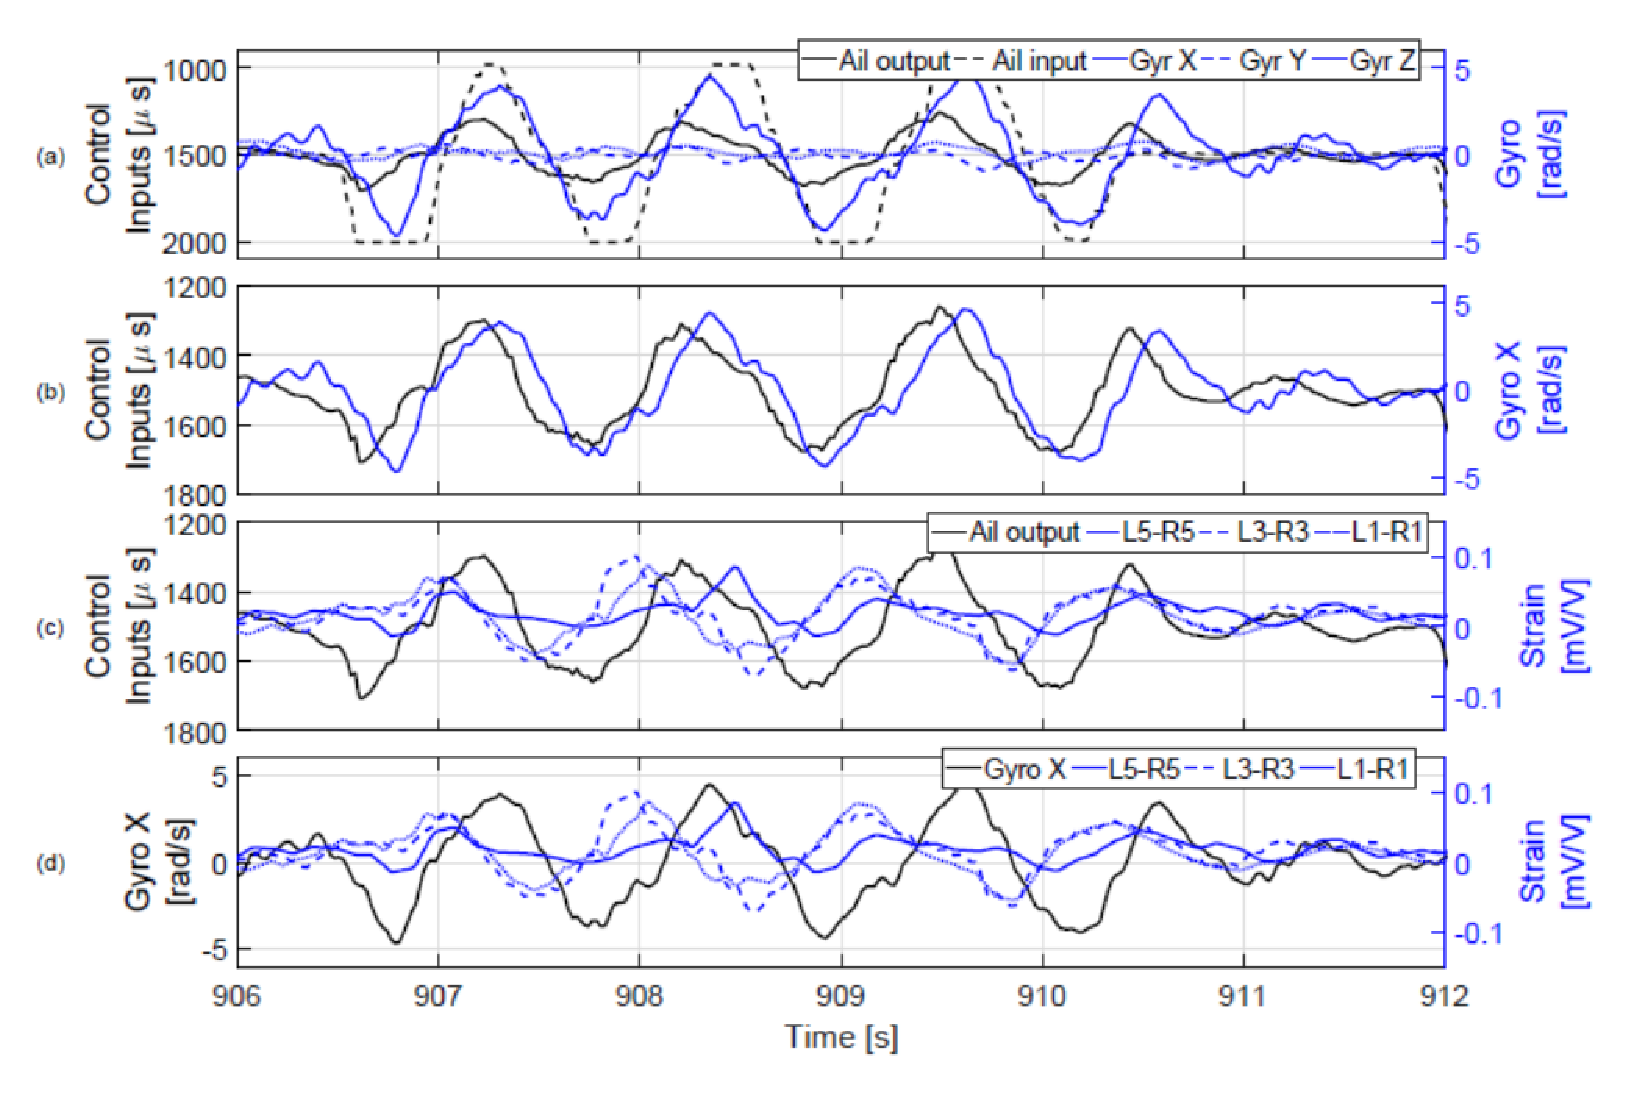
\includegraphics[width=\textwidth]{Strain_OutdoorsResponse2Controls.eps}};
		% Define scope with 'image' dimensions as reference
		\begin{scope}[x={(image.south east)},y={(image.north west)}]
			%\draw[help lines,xstep=.05,ystep=.05] (0,0) grid (1,1);
			%\foreach \x in {0,1,...,9} { \node [anchor=north] at (\x/10,0) {0.\x}; }
			%\foreach \y in {0,1,...,9} { \node [anchor=east] at (0,\y/10) {0.\y}; }
			
			\only<6>{
			  % Gyro Response
			  \draw(0.515,0.75) node[RectObject] (GyroResponse) {};
			  % Gyro Response label
			  \draw(0.515,0.30) node[LabelObject] (GyroResponse_Label)
				  {Gyro Response\\ to Aileron Command};
			  % Gyro Response arrow
			  \draw[ArrowObject] (GyroResponse_Label.north) -- (GyroResponse.south);
			}
			\only<7>{
			  % Gyro Response
			  \draw(0.515,0.315) node[RectObject] (StrainResponse) {};
			  % Gyro Response label
			  \draw(0.515,0.85) node[LabelObject] (StrainResponse_Label)
				  {Strain Response\\ to Aileron Command};
			  % Gyro Response arrow
			  \draw[ArrowObject] (StrainResponse_Label.south) -- (StrainResponse.north);
			}
			
		\end{scope}
  \end{tikzpicture}
}